\documentclass[../main.tex]{subfiles}
\begin{document}

\section{Multi-class classification  for VBF categorization}
\label{hh:sec:multiclass}

In the multi-class classification strategy, machine learning techniques are used to assign probability estimates for an event to belong to categories associated to any of the relevant physics processes under consideration.
The presence of several categories allows to study different signals with different topologies and to constrain nuisance parameters associated to backgrounds with large systematic uncertainties. By doing so, the analysis sensitivity can be enhanced.

In the HH$\to$bb$\tau\tau$ search, both of these characteristics are present. On the one hand, distinguishing between ggHH and VBFHH production helps to study the $\kappa_{2V}$ coupling strength, which is only available in the VBFHH production. On the other hand, the analysis is dominated by backgrounds, among the ones we find QCD multijet, Drell-Yan processes and processes involving the t quark (t$\bar{\text{t}}$ and t$\bar{\text{t}}$H). The first two have a big contribution thanks to its huge cross section, while the latter have a similar final state to the expected signal signature. Therefore, an strategy that discriminates between the signals and the different backgrounds could have a big effect in the final result.

\textcolor{red}{Fill with intro of the section: In section blabla, in section blabla...}

\subsection{Classification strategy}
\label{subs:hh:multi_class_strat}


Fig.~\ref{fig:hh:multi_approach} shows the concept of the event categorization using DNNs performing a multi-class classification, which can be described as follows. Per event, a predefined set of variables is used as input for a neural network whose architecture and weights are pre-trained and optimized. The network evaluates the variables and outputs for each event a vector of nine floating point numbers, each of them correspondent to the probability estimate for the event to be produced by the physical processes under consideration. In the HH$\to$bb$\tau\tau$ analysis, nine processes are defined. Three of them correspond to signal processes: $\text{HH}_{\text{ggF}}$, $\text{HH}_{\text{VBF}}$ produced with $\kappa_{2V}=1$ and a mixture of $\text{HH}_{\text{VBF}}$ produced with $\kappa_{2V}=0$ and $\kappa_{2V}=2$. Splitting the $\text{HH}_{\text{VBF}}$ contribution into a SM- and BSM-like component comes from the fact that the topology of the event differs a lot for different values of $\kappa_{2V}$. Therefore, considering only the $\text{HH}_{\text{VBF}}$ produced as in the SM could lead to an artificial bias of the network towards the SM topology, reducing the sensitivity when trying to exclude BSM scenarios. Regarding the background processes, the ones with the highest contribution (that were introduced before) are included. The contribution from t$\bar{\text{t}}$ is splitted according to the decays of the two W bosons into di-leptonic (DL), semi-leptonic (SL) and fully-hadronic (FH). t$\bar{\text{t}}$H is also included in two different samples, with the H decaying into b$\bar{\text{b}}$ or $\tau\bar{\tau}$, while an inclusive Z+jets sample is used to model the DY process. The QCD background, as described in Section~\ref{hh:subs:qcd}, is obtained in a data-driven way, so it can't be used as an output value by the DNN. Therefore, the six background processes previously described are the only ones we will consider.


\begin{figure}[h!]
\includegraphics[width=\textwidth]{Images/multiclass_approach}
\caption{Concept of the event categorization approach using a multi-class DNN. Every event is given nine floating point values, each of them expressing the probability of the event of being originated by the associated process. An event is categorized by the process class associated to the output with the highest value ($\text{HH}_{\text{ggF}}$ in the given example).}
\label{fig:hh:multi_approach}
\end{figure}

Each event, after obtaining its corresponding output values, is categorized by selecting the process whose corresponding node obtained the highest value. Nonetheless, the final categorization used in the analysis for signal extraction is obtained by merging some of the outputs: the three t$\bar{\text{t}}$, the two t$\bar{\text{t}}$H and the two $\text{HH}_{\text{VBF}}$ respectively. This way, only five distinct outputs remain: $\text{HH}_{\text{VBF}}$, $\text{HH}_{\text{ggF}}$, t$\bar{\text{t}}$, t$\bar{\text{t}}$H and DY. These merging could have been done initially by training and validating with 5 samples instead of 9. However, splitting the samples provides the network additional information on the underlying process, which can lead to a better training performance.

\subsection{Network architecture}

A representation of the neural network architecture is shown in Fig.~\ref{fig:hh:multi_architecture}. First, input variables are splitted into four-vector components of particles and higher-level variables. Four-vector variables are passed to a Lorentz Boost Network (LBN) \cite{hh:analysis:lbn}.
The purpose of this network is to extract high-level variables from four-vectors of particles and their combinations as part of the learning process. Together with the remaining input higher-level variables, they are forwarded to a standard, fully connected neural network that actually does the multi-class classification.

The final architecture used is the result of a hyperparameter optimization, and it will be described in Section~\ref{subs:hh:multi_training}.


\begin{figure}[h!]
\includegraphics[width=\textwidth]{Images/vbf_architecture}
\caption{Architecture of the multi-class classification network. Four-vector-like input features are passed through a Lorentz Boost Network for extracting high-level feature representations. These, together with the rest of input features, are forwarded to the actual neural network in order to do the classification of events.}
\label{fig:hh:multi_architecture}
\end{figure}

\subsection{Input variables}

Table~\ref{hh:fig:multi_variables} summarizes all variables considered as input to the neural network. Most of them are four-vector variables from different objects selected during the analysis: lepton (e, $\mu$ or $\tau_h$) candidates to be the decay product of one of the H, b jet candidates coming from the decays from the other H, VBF jets (if available), additional central jets not selected as the b jet candidates, forward jets not selected as the VBF jet candidates, MET and the $\text{H}_{\text{b}\bar{\text{b}}}$ and $\text{H}_{\tau\bar{\tau}}$ candidates. Additionally, some higher level features are included, such as the deep flavour and HH-btag scores for the b, VBF and additional central jets, and categorical features to provide information about the year of the input sample (so differences in detector alignment, trigger configurations or tuning parameters of the simulation can be inferred by the network) or the decay channel of the selected $\tau\tau$ pair.

\begin{table}[h!]
    \centering
    \footnotesize
      \begin{tabular}{|l|l|}
        \hline
        Variable name(s)                               & Description                                                                 \\
        \hline
        \texttt{is\_201\{6,7,8\}}                      & Flag denoting the campaign / year of input events.                          \\
        \texttt{is\_\{etau,mutau,tautau\}}             & Flag denoting reconstructed lepton channel.                                 \\
        \texttt{lep\{1,2\}\_\{e,pt,eta,phi\}}          & Four-vector components of the two leptons.                                  \\
        \texttt{bjet\{1,2\}\_\{e,pt,eta,phi\}}         & Four-vector components of the two b-tagged jets.                            \\
        \texttt{bjet\{1,2\}\_\{deepflavor,hhbtag\}}    & b-tag and HH-b-tag of the two b-tagged jets.                                \\
        \texttt{vbfjet\{1,2\}\_\{e,pt,eta,phi\}}       & Four-vector components of the two VBF jets.                                 \\
        \texttt{vbfjet\{1,2\}\_\{deepflavor,hhbtag\}}  & b-tag and HH-b-tag of the two VBF jets.                                     \\
        \texttt{ctjet\{1,2,3\}\_\{e,pt,eta,phi\}}      & Four-vector components of the three additional central jets.                \\
        \texttt{ctjet\{1,2,3\}\_\{deepflavor,hhbtag\}} & b-tag and HH-b-tag of the three additional central jets.                    \\
        \texttt{fwjet\{1,2\}\_\{e,pt,eta,phi\}}        & Four-vector components of the two additional forward jets.                  \\
        \texttt{met\_\{pt,phi\}}                       & Missing transverse energy and azimuthal direction.                          \\
        \texttt{bh\_\{e,pt,eta,phi\}}                  & Four-vector components of the reconstructed $H_{b\bar{b}}$ candidate.       \\
        \texttt{tauh\_\{e,pt,eta,phi\}}                & Four-vector components of the reconstructed $H_{\tau\bar{\tau}}$ candidate. \\
        \hline
      \end{tabular}
     \caption{Names and descriptions of variables considered as inputs to the neural network.}
    \label{hh:fig:multi_variables}
\end{table}


\textcolor{red}{Shall we include input variable plots?}


\subsection{Training procedure and network optimization}
\label{subs:hh:multi_training}

To perform the training and validation of the DNN, events from 2016, 2017 and 2018 passing the VBF category selection (described in Section \ref{hh:sec:event_categorization}) are considered. In order to exploit the full amount of events without introducing a potential bias on the DNN outputs due to overtraining, a two-fold cross validation approach is performed: the available simulated events are divided into two independent datasets, the ones with \textit{even} event numbers and the ones with \textit{odd} event numbers. This way, the network trained and validated with even event numbers will be used for infering the DNN outputs for the events with odd event numbers and vice versa. On each dataset, a dedicated training is performed using 70\% for the actual training, while 30\% is used to perform the immediate cross validation. To increase the statistical robustness, ensembles of ten networks with different random seeds are trained and merged with the same weight after each particular training finishes, so the final outputs of the DNN inference are the average of the 10 DNN outputs.

Training is performed with the \textsc{Tensorflow} \cite{hh:analysis:tensorflow} algorithm interfaced with \textsc{Keras} \cite{hh:analysis:keras} and independently for even and odd event numbers. In fact, a hyperparameter optimization is performed for each network via a grid-based scanning procedure, so the networks for even and odd event numbers could end up being totally different. The results of these optimizations, however, lead to only slightly different networks. In both cases, the optimal network contains four hidden layers, each with 128 units and $\tanh$ as activation function, and an output layer with nine units subject to a softmax activation function (so the DNN scores take values between 0 and 1 and sum 1). The training with even (odd) event numbers was performed using the Adam optimizer with a learning rate of 0.001 (0.006), an $\text{L}_2$ normalization factor $\lambda$ of $5(2)\times 10^{-5}$ and a common batch size of 1024, equally populated by the nine physics processes under investigation. During the training, the method of batch normalization is applied as well as a random unit dropout with a probability of 5\%. The loss function in both cases is constructed as a sum of three individual loss terms,
\begin{equation}
 L(y(x), y_G(x), \hat{y}, \hat{y}_G)_\text{CE} = \frac{1}{N} \sum_n^N -\hat{y}_n \log{y_n(x)} \hspace{2mm} + \hspace{2mm} \frac{1}{N} \sum_n^N -\hat{y}_{G,n} \log{y_{G,n}(x)} \hspace{2mm} + \hspace{2mm} L_2(\lambda),
\end{equation}
where the first two terms represent categorical cross entropy (CE) functions and the third term a typical $\text{L}_2$ normalization (to keep the model weights as small as possible) factorized by $\lambda$. The first CE is applied to all nine output classes and compares the prediction $y_n(x)$ of an event $n$ given the inputs $x$ with the true value $\hat{y}_n$. For the second CE, outputs are combined into a signal class (all HH processes) and a background class. This increases the relative importance of signal events and balances the importance of an HH event of a given class being classified as an event from a different signal class (and analogously for background events). Given the analysis strategy with three different signal definitions, it should be beneficial to do this kind of balancing. This second CE term is often called \textit{grouped} cross entropy.



\subsection{Training and validation results}

Fig.~\ref{hh:fig:multi_roc} shows the ROC curves of the trained networks with even and odd numbers separately for training and validation events. No significant differences between the training and validation datasets, then overtraining has been sufficiently suppressed. The separation performance of the training networks can be seen in the large area-under-curve (AUC) values, above 0.93 for HH signals and between 0.75-0.95 for backgrounds.

\begin{figure}[h!]
\begin{center}
\subfloat[Training data, even event numbers]{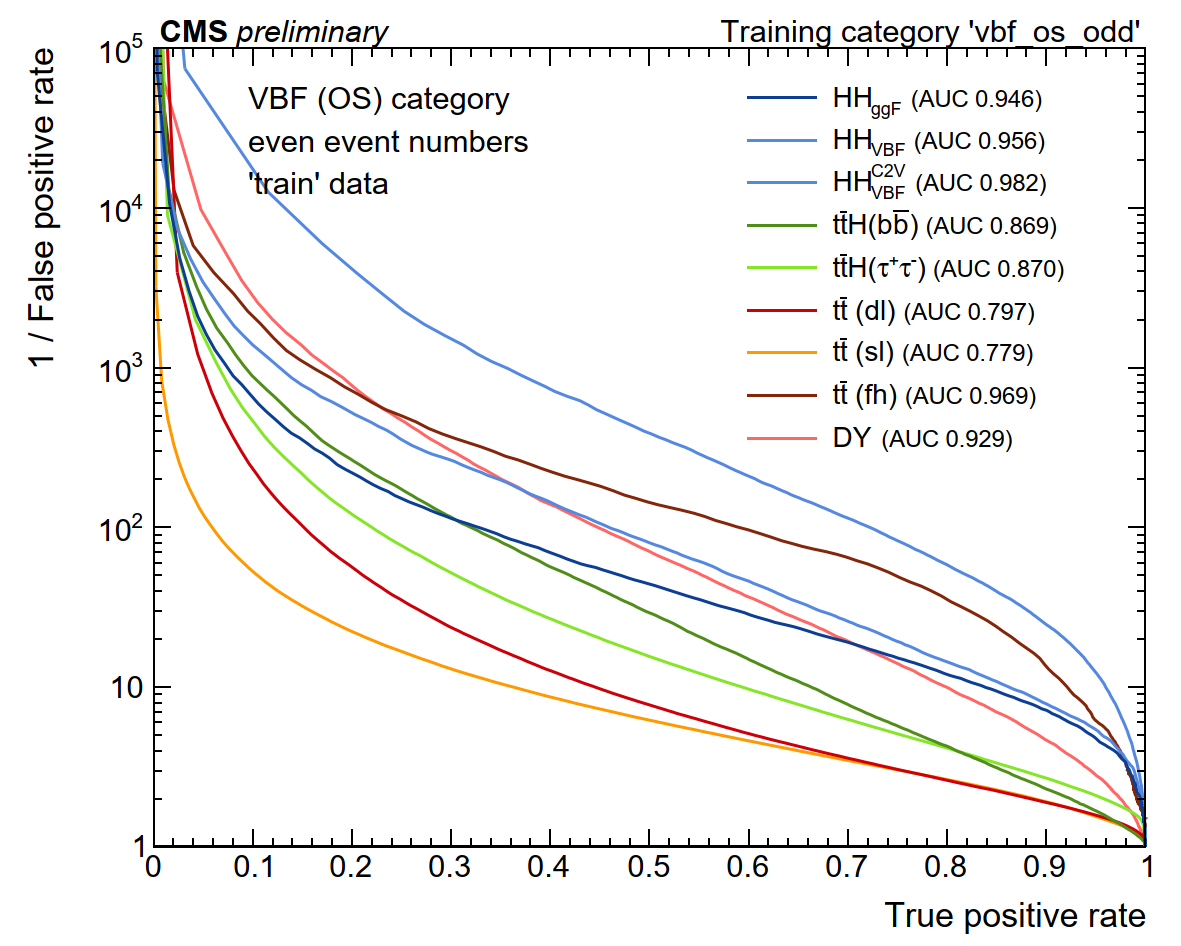
\includegraphics[width=0.45\textwidth]{Images/roc__run2__train__even}}
\subfloat[Validation data, even event numbers]{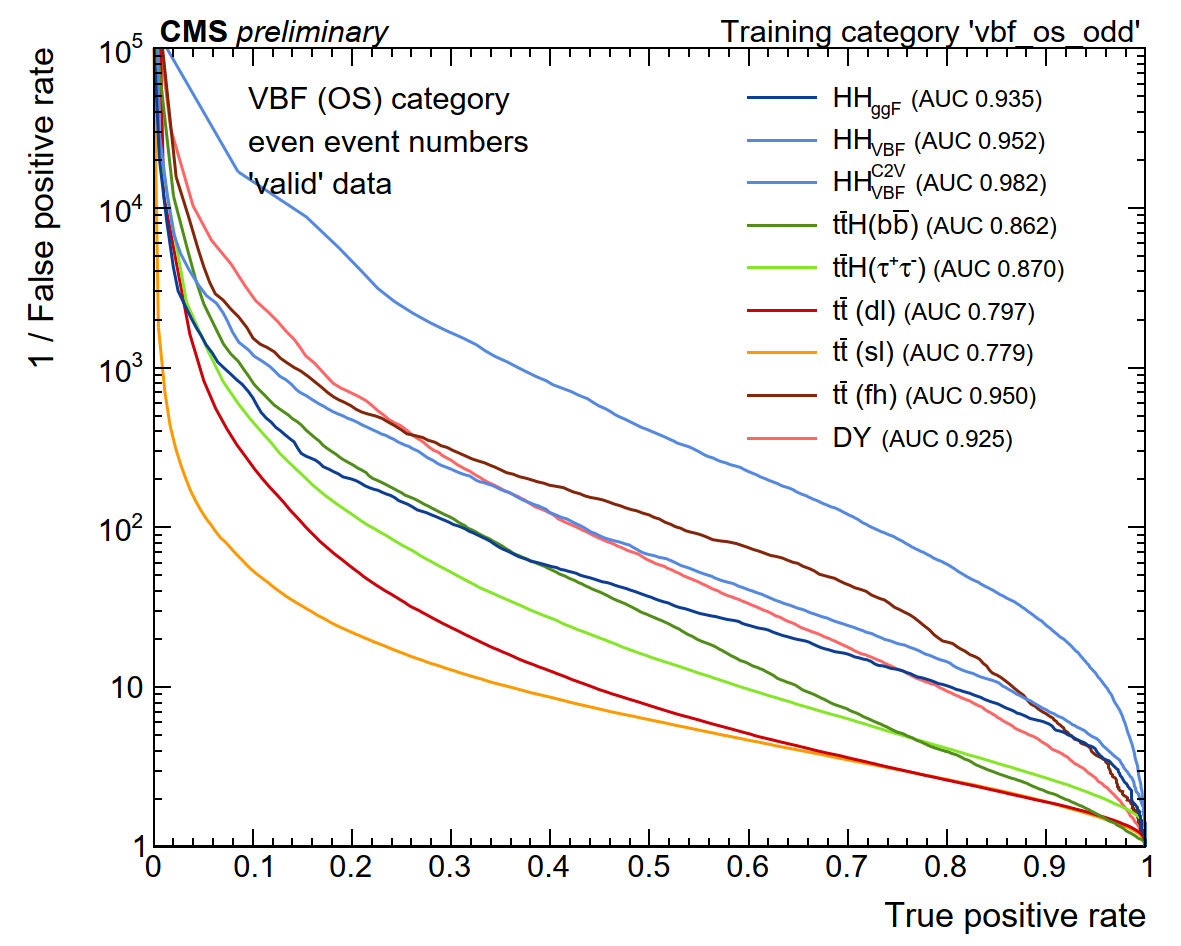
\includegraphics[width=0.45\textwidth]{Images/roc__run2__valid__even}} \\
\subfloat[Training data, odd event numbers]{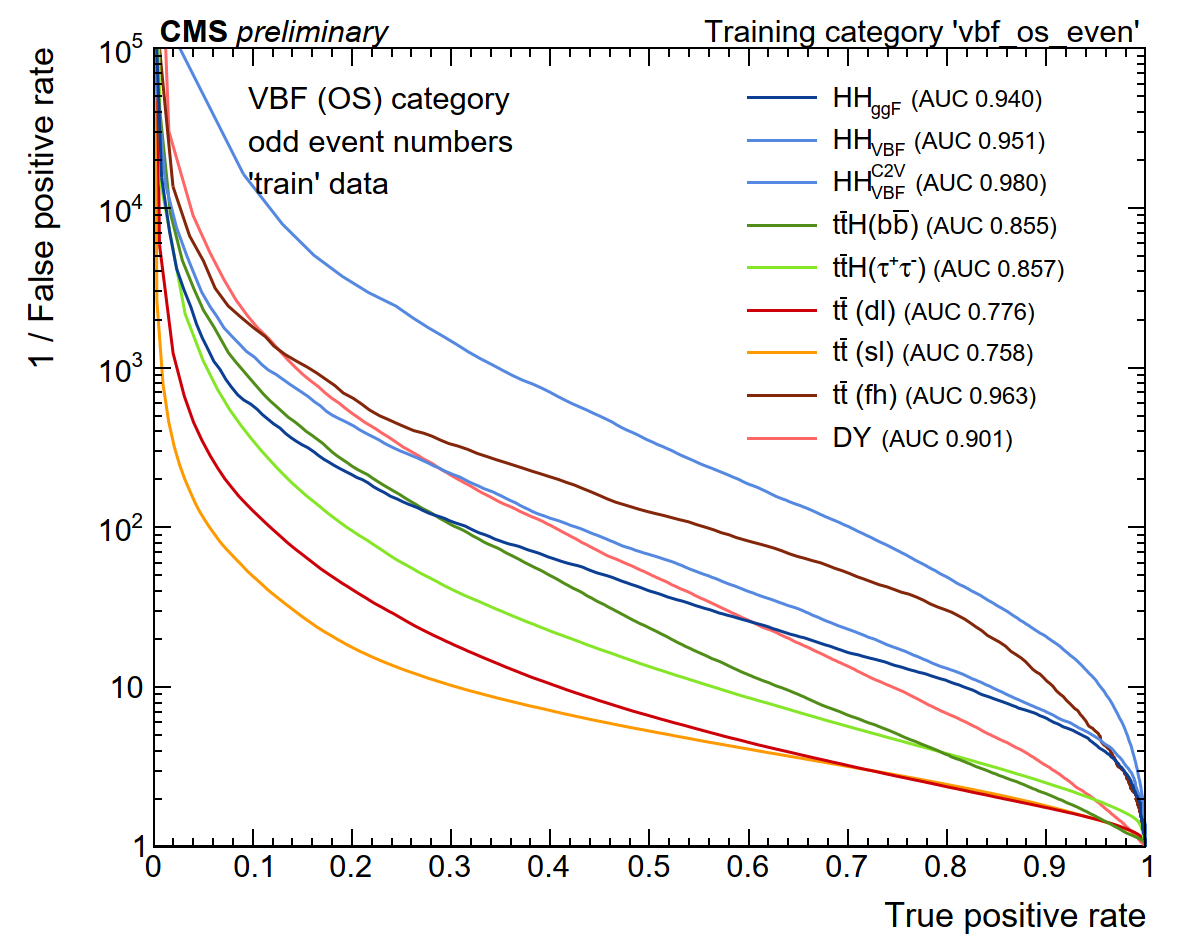
\includegraphics[width=0.45\textwidth]{Images/roc__run2__train__odd}}
\subfloat[Validation data, odd event numbers]{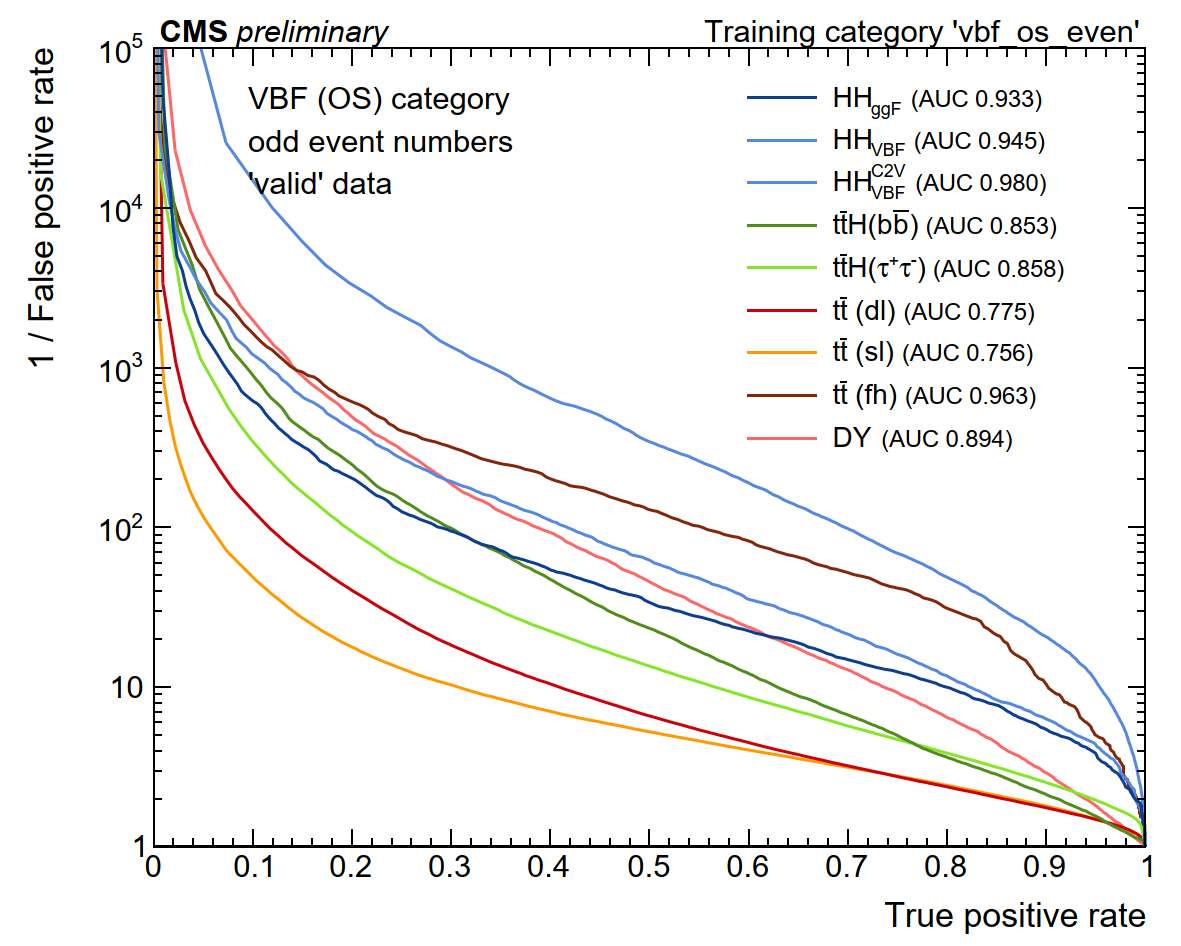
\includegraphics[width=0.45\textwidth]{Images/roc__run2__valid__odd}}
\end{center}
\caption{ROC curves showing the relation between true and false positive rates, evaluated for a particular process against all others separately on the training (left) and validation (right) data and for even (top) and odd (bottom) event numbers. Corresponding area-under-curve values are shown in the legend.}
\label{hh:fig:multi_roc}
\end{figure}

The efficiency of the categorization achieved by this approach can be seen in the so-called confusion matrices shown in Fig.~\ref{hh:fig:multi_confusion}. Numbers are normalized per row, and represent the probability of an event to have its process correctly predicted or not. Accuracies are denoted by the diagonal, while off-diagonal values correspond to confusion rates. Note how most of the signal events stay in the signal categories, while very little background contamination can be observed in these categories. A sixth row has been added in the matrices containing QCD events obtained by the data-driven method. Even if the training was not performed with the QCD process as input, QCD events get classified mostly in background categories, with little contamination affecting the HH${}_\text{VBF}$ category.



\begin{figure}[h!]
\begin{center}
\subfloat[2016]{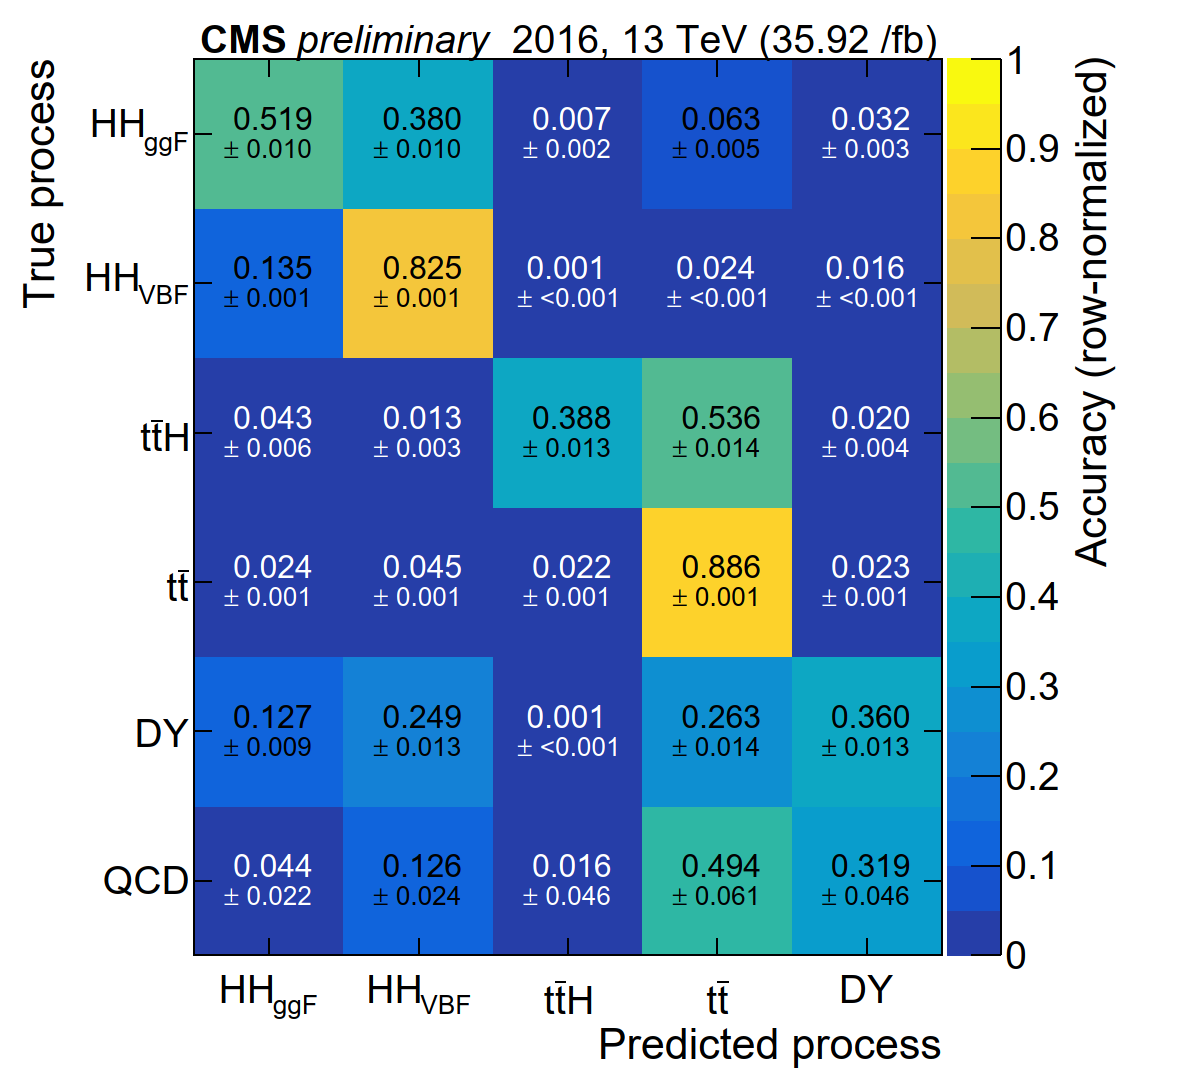
\includegraphics[width=0.45\textwidth]{Images/confusion__2016__nodata}}
\subfloat[2017]{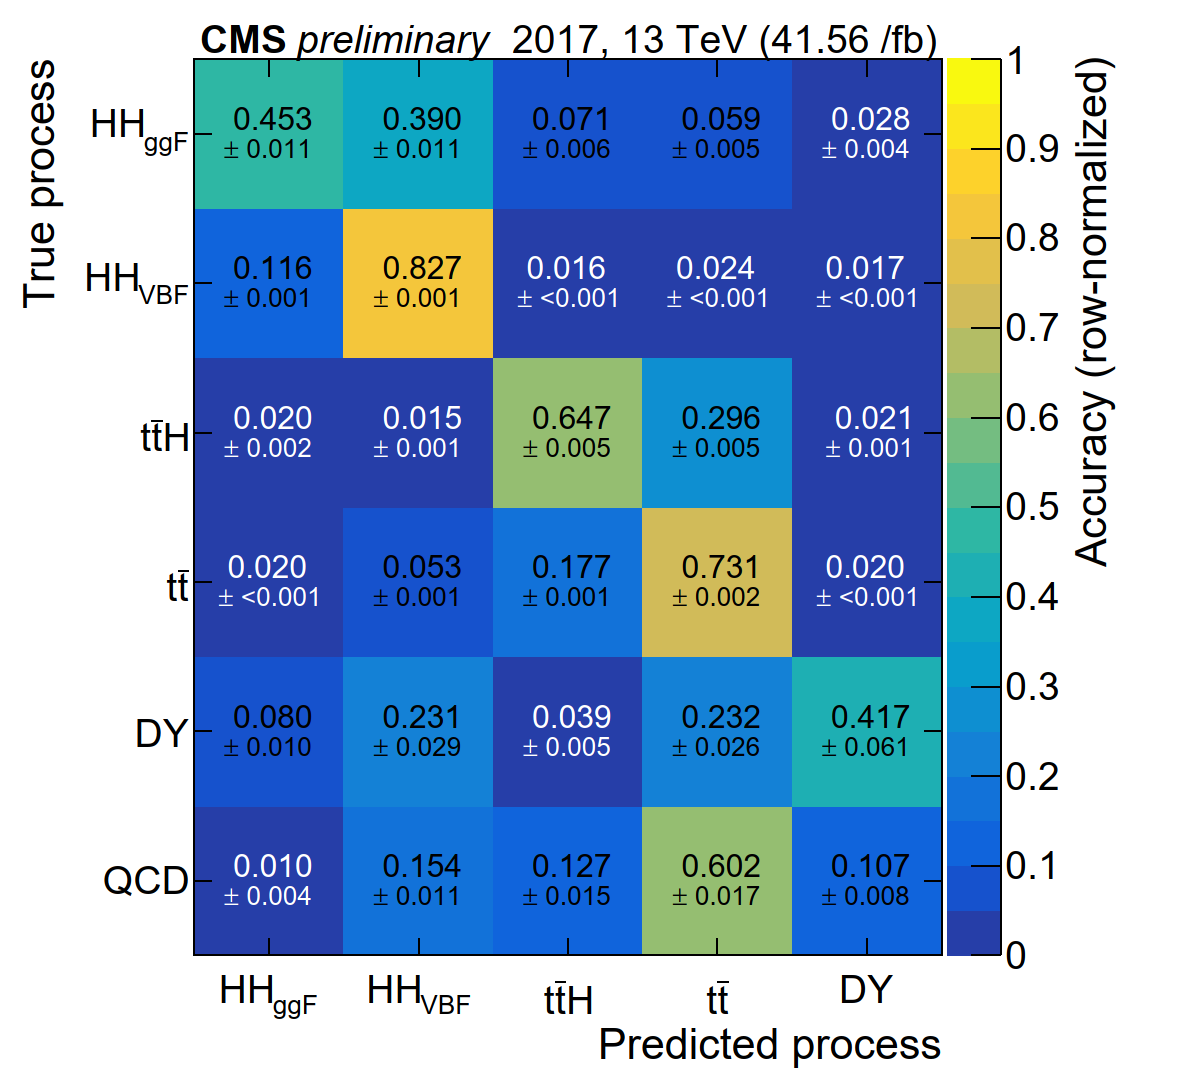
\includegraphics[width=0.45\textwidth]{Images/confusion__2017__nodata}} \\
\subfloat[2018]{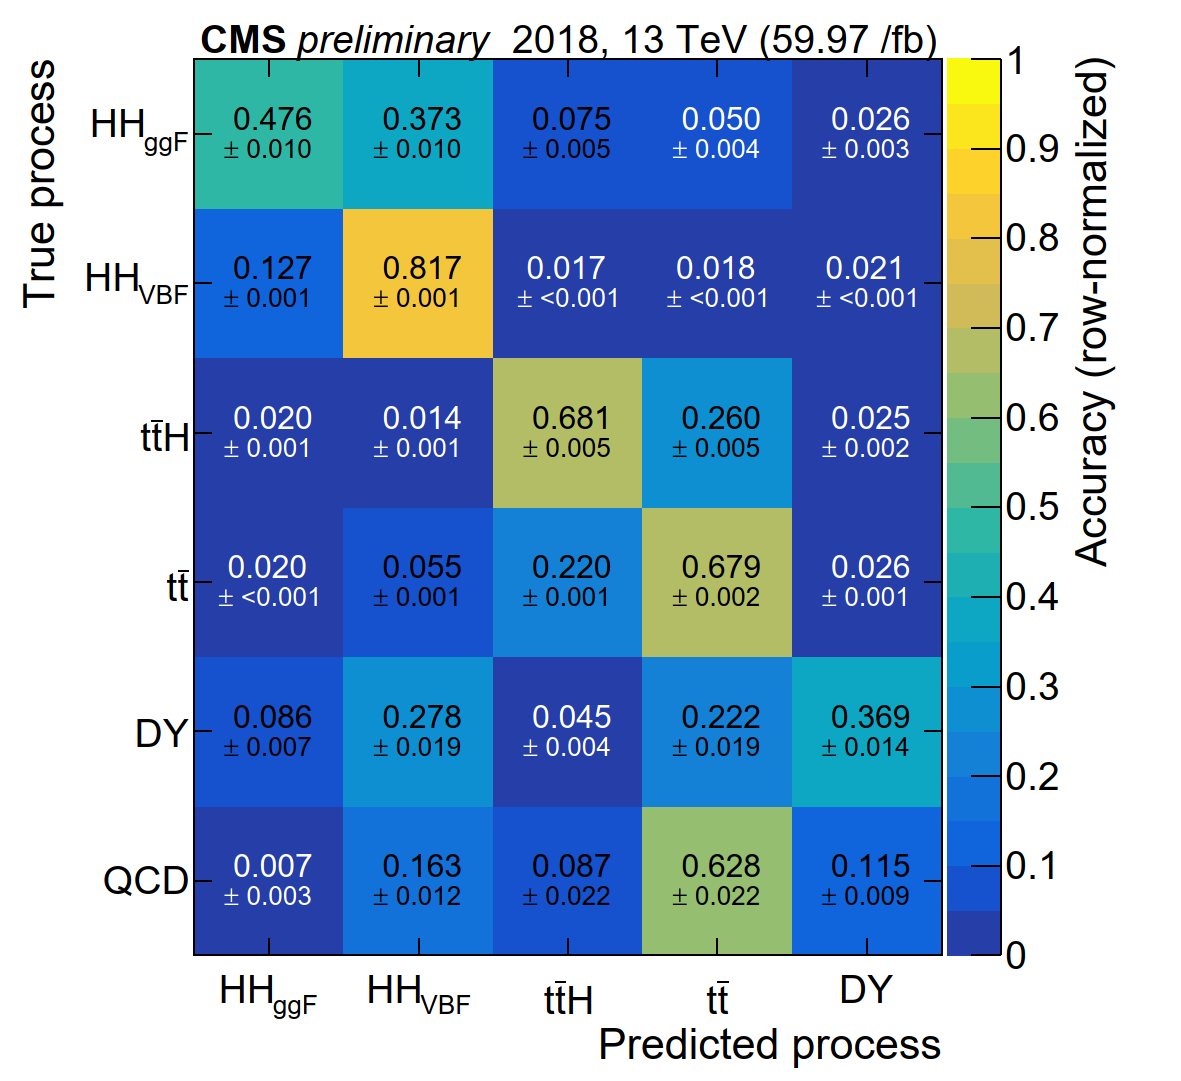
\includegraphics[width=0.45\textwidth]{Images/confusion__2018__nodata}}
\end{center}
\caption{Row-normalized process classification accuracies and confusion rates, evaluated for the three data-taking years. Note that the two $\text{HH}_{\text{VBF}}$, the two t$\bar{\text{t}}$H and the three t$\bar{\text{t}}$ processes are merged following the categorization strategy described in Section \ref{subs:hh:multi_class_strat}.}
\label{hh:fig:multi_confusion}
\end{figure}


%\bibliographystyle{unsrt}
%\bibliography{../biblio.bib}


\end{document}

